\onecolumn
\chapter{Auswertung}
\label{ch:auswertung}

\section*{Fehlerrechnung}
Für die statistische Auswertung von $n$ Messwerten $x_i$ werden folgende Größen definiert \cite{errorSkript25}:
\begin{align}
    \bar{x} &= \frac{1}{n} \sum_{i=1}^{n} x_i \vphantom{\sqrt{\sum_i^n}^2} && \text{\textcolor{gray}{Arithmetisches Mittel}} \label{eq:arithmetisches_mittel} \\
    \sigma^2 &= \frac{1}{n-1} \sum_{i=1}^{n} (x_i - \bar{x})^2 \vphantom{\sqrt{\sum_i^n}^2} && \text{\textcolor{gray}{Variation}} \label{eq:variation} \\
    \sigma &= \sqrt{\frac{1}{n-1} \sum_{i=1}^{n} (x_i - \bar{x})^2} \vphantom{\sqrt{\sum_i^n}^2} && \text{\textcolor{gray}{Standardabweichung}} \label{eq:standardabweichung} \\
    \Delta \bar{x} &= \frac{\sigma}{\sqrt{n}} = \sqrt{\frac{1}{n(n-1)} \sum_{i=1}^n(\bar x - x_i)^2} \vphantom{\sqrt{\sum_i^n}^2} && \text{\textcolor{gray}{Fehler des Mittelwerts}} \label{eq:fehler_mittelwert} \\
    \Delta f &= \sqrt{\left(\frac{\partial f}{\partial x} \Delta x\right)^2 + \left(\frac{\partial f}{\partial y} \Delta y\right)^2} \vphantom{\sqrt{\sum_i^n}^2} && \text{\textcolor{gray}{Gauß’sches Fehlerfortpflanzungsgesetz für $f(x,y)$}} \label{eq:gauss_fehlfortpflanzung} \\
    \Delta f &= \sqrt{(\Delta x)^2 + (\Delta y)^2} \vphantom{\sqrt{\sum_i^n}^2} && \text{\textcolor{gray}{Fehler für $f = x + y$}} \label{eq:fehler_summe} \\
    \Delta f &= |a| \Delta x \vphantom{\sqrt{\sum_i^n}^2} && \text{\textcolor{gray}{Fehler für $f = ax$}} \label{eq:fehler_proportional} \\
    \frac{\Delta f}{|f|} &= \sqrt{\left(\frac{\Delta x}{x}\right)^2 + \left(\frac{\Delta y}{y}\right)^2} \vphantom{\sqrt{\sum_i^n}^2} && \text{\textcolor{gray}{relativer Fehler für $f = xy$ oder $f = x/y$}} \label{eq:relativer_fehler} \\
    \sigma &= \frac{|a_{lit} - a_{gem}|}{\sqrt{\Delta a_{lit}^2 + \Delta a_{gem}^2}} \vphantom{\sqrt{\sum_i^n}^2} && \text{\textcolor{gray}{Berechnung der signifikanten Abweichung}} \label{eq:signifikante_abweichung}
\end{align}

\twocolumn

\section{Molarextintion über die Lambert-Gerade}
Für folgende Rechnung liegen die Werte der Tabelle 1 des \hyperref[Protokoll]{Protokolls} zugrunde. Aus diesen soll die Molarextintion über die Lambert-Gerade bstimmt werden. Hierfür wird die gemessene Intensität gegen die Schichtdicke des Kaliumpermanganat geplottet. Dies wird auf halblogarithmischen papier gemacht. Zunächst muss die Ungenauigkeit der Intensität bestimmt werden, dies geschieht über die \hyperref[eq:gauss_fehlfortpflanzung]{Gauß'sche Fehlerfortpflanzung (\ref*{eq:gauss_fehlfortpflanzung})} der \hyperref[eq:correction]{Gleichung \ref*{eq:correction}}:
\begin{equation}
    \hspace{-0.25cm}
    \frac{\Delta I_{\text{korr}}}{I_{\text{korr}}} = \sqrt{\left(\frac{\Delta I}{I}\right)^2 + \left(\frac{2 \Delta D_{\text{mK}}}{D_{\text{mK}}}\right)^2 + \left(\frac{2 \Delta D_{\text{oK}}}{D_{\text{oK}}}\right)^2}
\end{equation}


Dies ist der Fehler der längsten Küvette (25cm). Die Abbildunsggröße betrug dabei $(22,0 \pm 1,4) \mathrm{mm}$. Die Intensität ist der Mittelwert der 5 Einzelmessungen Somit kommt man auf eine Ungenauigkeit von:
\begin{equation}
    I_{\text{korr}} = 280 \pm 60
\end{equation}

Die Werte der Tabelle 1 des pp nochmal schön aufgetragen, mit korrigierten \hyperref[eq:fehler_mittelwert]{Fehler des Mittelwerts (\ref*{eq:fehler_mittelwert})}:
\begin{table}[b!]
    \onecolumn
    \centering
    \begin{tabular}{l | ccccc}
    \hline
    Nr. & Probe 1 & Probe 2 & Probe 3 & Probe 4 & Probe 5 \\
    \hline
    1 & 57986,15 & 42025,17 & 20706,55 & 3785,81 & 238,52 \\
    2 & 58064,89 & 42039,61 & 20728,90 & 3785,01 & 236,01 \\
    3 & 58051,22 & 42059,49 & 20698,69 & 3783,42 & 234,55 \\
    4 & 58091,77 & 42055,26 & 20696,26 & 3770,97 & 236,08 \\
    5 & 58038,11 & 42051,74 & 20700,11 & 3782,10 & 234,51 \\
    \hline
    $\bar{x} \pm \Delta \bar{x}$ & 58046 $\pm$ 16 & 42046 $\pm$ 6 & 20706 $\pm$ 5 & 3781,5 $\pm$ 2,4 & 235,9 $\pm$ 0,7 \\
    \hline
    \end{tabular}
    \caption{Messwerte der fünf Proben mit Mittelwert und Standardfehler des Mittelwerts (SEM).}
    \twocolumn
\end{table}

Die Ergebnisse sind in \hyperref[fig:g_l]{Abbildung \ref*{fig:g_l}} dargestellt. Mit den \hyperref[eq:beer]{Gleichungen \ref*{eq:beer} und \ref*{eq:combined}} ergibt sich:

\begin{equation}
\frac{\lg(I_0) - \lg(I(l))}{l} = k'
\end{equation}

Damit sind die Steigungen der beiden geraden:
\begin{align}
    {k_A}' &= \frac{\lg(60\,000) - \lg(95)}{28,85\mathrm{cm}} = -0,09707 \, \frac{1}{\mathrm{cm}}\\
    {k_F}' &= \frac{\lg(58\,056) - \lg(220)}{22,5\mathrm{cm}} = -0,10762 \, \frac{1}{\mathrm{cm}}
\end{align}

Damit ergibt sich:
\begin{equation}
\boxed{
    k' = (0,0971\pm 0,0106) \, \frac{1}{\mathrm{cm}}
}
\end{equation}

Nun \hyperref[eq:beer]{Gleichung \ref*{eq:beer}} nach $\epsilon$ umformen und \hyperref[eq:gauss_fehlfortpflanzung]{Gauß'sche Fehlerfortpflanzung (\ref*{eq:gauss_fehlfortpflanzung})} anwenden:
\begin{equation}
    \Delta \epsilon = \frac{\Delta k'}{c}
\end{equation}

Daraus ergibt sich bei einer Konzentration von $c = 5 \cdot 10^{-5} \, \mathrm{\frac{mol}{l}}$:
\begin{equation}
\boxed{
    \epsilon = (1900 \pm 200) \, \mathrm{\frac{cm^2}{mol}}
}
\end{equation}

\onecolumn
\begin{figure}
    % \hspace{-2.2cm}
    \includegraphics[width=1\textwidth]{img/34/g1--34–Spektralfotometrie.pdf}
    \caption{Ausgelichsgerade (blau) und Fehlergerade (orange) der Messwerte aus Tabelle 1 für das Lambert-Verfahren}
    \label{fig:g_l}
\end{figure}
\twocolumn

\section{Molarextintion über die Beer-Gerade}
In dieser Sektion wird die molare Extinktion mithilfe der Beer’schen Gerade berechnet. Dazu werden die Intensitäten aus Tabelle 2 des \hyperref[Protokoll]{Protokolls} als Funktion der Konzentration \( c \) der verwendeten Lösung dargestellt. Die Konzentrationen ergeben sich aus den Messprotokollangaben; die entsprechenden Werte sind bereits im Praktikumsskript enthalten \cite{skript25}. Zusätzlich muss für jede Konzentration der zugehörige Fehler bestimmt werden.

Der allgemeine Ausdruck für den Fehler \(\Delta c_i\) lautet:

\begin{equation}
\Delta c_i = \tilde{c} \frac{1}{V_{\text{ges}}^2}
\left(
V_0^2 \sum_{j=1}^{i} \Delta V_j^2 + (V_{\text{ges}} - V_0)^2 \Delta V_0^2
\right)^{\frac{1}{2}}
\end{equation}

Dabei ist \(\tilde{c} = 10^{-3}\,\text{mol/l}\) die Konzentration der Kaliumpermanganat-Lösung in der Bürette, mit der die Küvette befüllt wird. Der Volumenfehler \(\Delta V_j\) ist dem Messprotokoll zu entnehmen.

Das Gesamtvolumen \(V_{\text{ges}}\) der Lösung ergibt sich zu:

\begin{equation}
V_{\text{ges}} = \sum_{j=0}^{i} V_j
\end{equation}

Die Ergebnisse sind \hyperref[tab:beer]{tabellarisch \ref*{tab:beer}} festgehalten.
\begin{table}[!ht]
    \centering
    \begin{tabular}{l | c | c}
        \toprule
        Nr. & $c_i {\mathrm{\frac{mol}{l}} \cdot 10^{-4}}$ & Itensität \\
        \hline
        1 & $0,0 \pm 0,0$ & $57830 \pm 16$ \\
        2 & $0,63 \pm 0,06$ & $31597 \pm 5$ \\
        3 & $1,25 \pm 0,07$ & $16905 \pm 8$ \\
        4 & $2,5 \pm 0,07$ & $4342 \pm 4$ \\
        5 & $5 \pm 0,04$ & $234,86 \pm 1,05$ \\         
        \bottomrule
    \end{tabular}
    \label{tab_beer}
    \caption{Ergebniss der Konzentrationen und der gemessenen Itensitäten.}
\end{table}

Aus \hyperref[fig:g_2]{Abbildung \ref*{fig:g_2}} sind die Steigungen 
\begin{align}
    m_A &= -6950,61728 \, \mathrm{\frac{l}{mol}}\\
    m_F &= -11523,77183 \, \mathrm{\frac{l}{mol}}
\end{align}

somit ergibt sich eine Steigungen:
\begin{equation}
\boxed{
    m = -(7000 \pm 5000) \, \mathrm{\frac{l}{mol}}
}
\end{equation}

Für das $\epsilon$ ergibt sich über
\begin{equation}
\epsilon_B = \frac{s}{l} 
\end{equation}

und seinem Fehler 
\begin{equation}
\Delta \epsilon_B = \frac{\Delta  s}{l} 
\end{equation}

folglich bei einer dicke von $l = 1,5$ cm:

\begin{equation}
\boxed{
    \epsilon_B = (5000 \pm 3000) \cdot 10^3 \mathrm{\frac{cm^2}{mol}}
}
\end{equation}

\section{Abweichung der Ergebnisse}
Zuletzt wird die \hyperref[eq:signifikante_abweichung]{signifikante Abweichung (\ref*{eq:signifikante_abweichung})} berehnet:
\begin{equation}
    \frac{\left| \epsilon_L - \epsilon_B \right|}{\sqrt{(\delta \epsilon_L)^2 + (\delta \epsilon_B)^2}} = 1,03\sigma
\end{equation}

\onecolumn
\begin{figure}
    % \hspace{-2.2cm}
    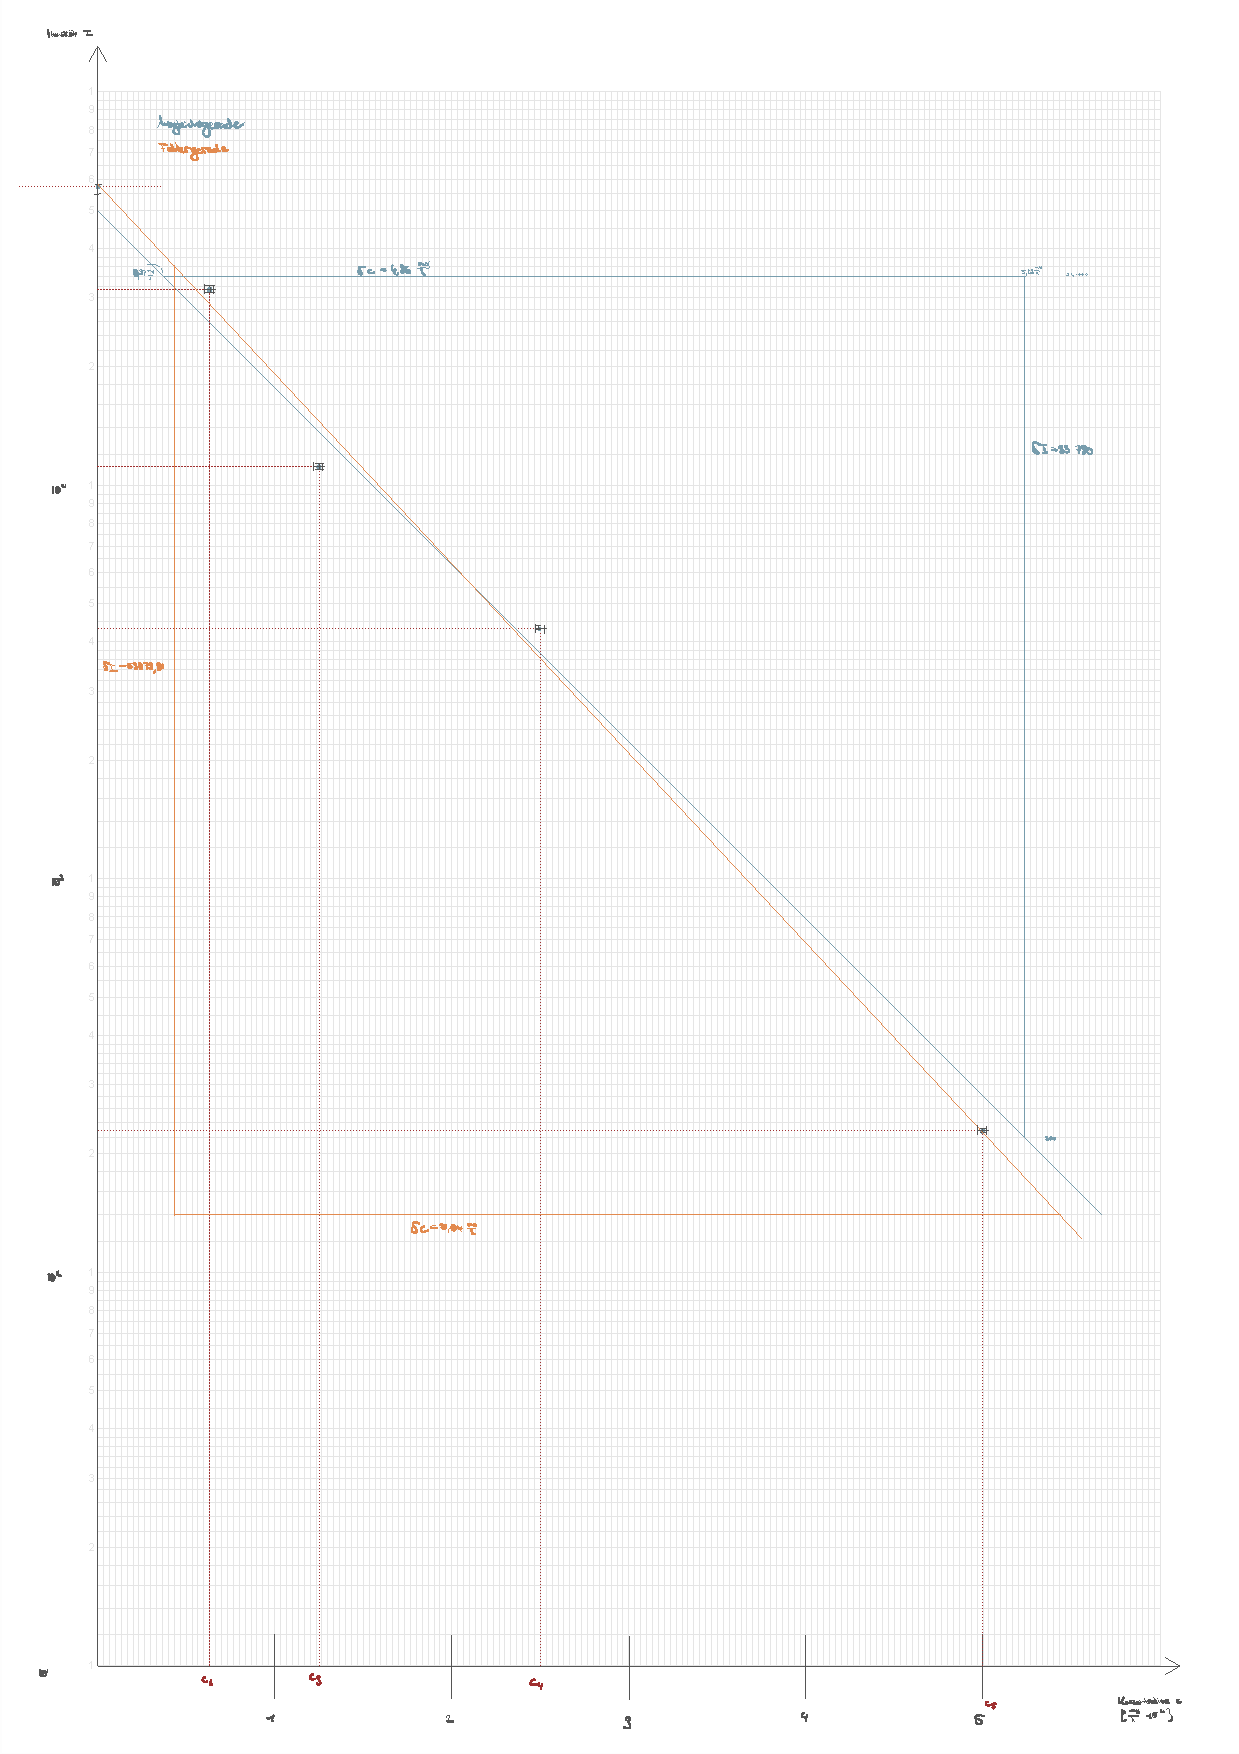
\includegraphics[width=1\textwidth]{img/34/g2--34-Spektralfotometrie.pdf}
    \caption{Ausgelichsgerade (blau) und Fehlergerade (orange) der Messwerte aus Tabelle 1 für das Lambert-Verfahren}
    \label{fig:g_2}
\end{figure}
\twocolumn